\documentclass[12pt,a4paper]{article}
\usepackage{amsmath,amssymb,mathrsfs,tikz,times,pifont}
\usepackage{enumitem}
\newcommand\circitem[1]{%
\tikz[baseline=(char.base)]{
\node[circle,draw=gray, fill=red!55,
minimum size=1.2em,inner sep=0] (char) {#1};}}
\newcommand\boxitem[1]{%
\tikz[baseline=(char.base)]{
\node[fill=cyan,
minimum size=1.2em,inner sep=0] (char) {#1};}}
\setlist[enumerate,1]{label=\protect\circitem{\arabic*}}
\setlist[enumerate,2]{label=\protect\boxitem{\alph*}}
%%%::::::by chnini ameur :::::::%%%
\everymath{\displaystyle}
\usepackage[left=1cm,right=1cm,top=1cm,bottom=1.7cm]{geometry}
\usepackage{array,multirow}
\usepackage[most]{tcolorbox}
\usepackage{varwidth}
\usepackage{tkz-tab}
\tcbuselibrary{skins,hooks}
\usetikzlibrary{patterns}
%%%::::::by chnini ameur :::::::%%%
\newtcolorbox{exa}[2][]{enhanced,breakable,before skip=2mm,after skip=5mm,
colback=yellow!20!white,colframe=black!20!blue,boxrule=0.5mm,
attach boxed title to top left ={xshift=0.6cm,yshift*=1mm-\tcboxedtitleheight},
fonttitle=\bfseries,
title={#2},#1,
% varwidth boxed title*=-3cm,
boxed title style={frame code={
\path[fill=tcbcolback!30!black]
([yshift=-1mm,xshift=-1mm]frame.north west)
arc[start angle=0,end angle=180,radius=1mm]
([yshift=-1mm,xshift=1mm]frame.north east)
arc[start angle=180,end angle=0,radius=1mm];
\path[left color=tcbcolback!60!black,right color = tcbcolback!60!black,
middle color = tcbcolback!80!black]
([xshift=-2mm]frame.north west) -- ([xshift=2mm]frame.north east)
[rounded corners=1mm]-- ([xshift=1mm,yshift=-1mm]frame.north east)
-- (frame.south east) -- (frame.south west)
-- ([xshift=-1mm,yshift=-1mm]frame.north west)
[sharp corners]-- cycle;
},interior engine=empty,
},interior style={top color=yellow!5}}
%%%%%%%%%%%%%%%%%%%%%%%

\usepackage{fancyhdr}
\usepackage{eso-pic}         % Pour ajouter des éléments en arrière-plan
% Commande pour ajouter du texte en arrière-plan
\AddToShipoutPicture{
    \AtTextCenter{%
        \makebox[0pt]{\rotatebox{80}{\textcolor[gray]{0.7}{\fontsize{5cm}{5cm}\selectfont PGB}}}
    }
}
\usepackage{lastpage}
\fancyhf{}
\pagestyle{fancy}
\renewcommand{\footrulewidth}{1pt}
\renewcommand{\headrulewidth}{0pt}
\renewcommand{\footruleskip}{10pt}
\fancyfoot[R]{
\color{blue}\ding{45}\ \textbf{2025}
}
\fancyfoot[L]{
\color{blue}\ding{45}\ \textbf{Prof:M. BA}
}
\cfoot{\bf
\thepage /
\pageref{LastPage}}
\begin{document}
\renewcommand{\arraystretch}{1.5}
\renewcommand{\arrayrulewidth}{1.2pt}
\begin{tikzpicture}[overlay,remember picture]
\node[draw=blue,line width=1.2pt,fill=purple,text=blue,inner sep=3mm,rounded corners,pattern=dots]at ([yshift=-2.5cm]current page.north) {\begingroup\setlength{\fboxsep}{0pt}\colorbox{white}{\begin{tabular}{|*1{>{\centering \arraybackslash}p{0.28\textwidth}} |*2{>{\centering \arraybackslash}p{0.2\textwidth}|} *1{>{\centering \arraybackslash}p{0.19\textwidth}|} }
\hline
\multicolumn{3}{|c|}{$\diamond$$\diamond$$\diamond$\ \textbf{Lycée de Dindéfélo}\ $\diamond$$\diamond$$\diamond$ }& \textbf{A.S. : 2024/2025} \\ \hline
\textbf{Matière: Mathématiques}& \textbf{Niveau : 2nd}\textbf{L} &\textbf{Date: 19/03/2025} & \textbf{Durée : 3 heures} \\ \hline
\multicolumn{4}{|c|}{\parbox[c]{10cm}{\begin{center}
\textbf{{\Large\sffamily Correction du devoir n$ ^{\circ} $ 1 du 2$ ^\text{\bf nd} $ Semestre}}
\end{center}}} \\ \hline
\end{tabular}}\endgroup};
\end{tikzpicture}
\vspace{3cm}

\section*{\underline{Exercice 1 :} 6 points ( Développement, Réduction et Factorisation )}

\begin{enumerate}
\item Développons et réduisons les expressions données :
\begin{align*}
\textbf{A}(x) &= (2x - 3)(4x^2 + 6x + 9) \\ 
  &= 2x \cdot (4x^2 + 6x + 9) - 3 \cdot (4x^2 + 6x + 9) \\ 
  &= (2x \cdot 4x^2) + (2x \cdot 6x) + (2x \cdot 9) - (3 \cdot 4x^2) - (3 \cdot 6x) - (3 \cdot 9) \\ 
  &= 8x^3 + 12x^2 + 18x - 12x^2 - 18x - 27 \\ 
  &= 8x^3 + (12x^2 - 12x^2) + (18x - 18x) - 27 \\ 
  &= 8x^3 - 27.
\end{align*}
$$\textcolor{red}{\boxed{E=8x^3 - 27}}$$

\begin{align*}
\textbf{B}(x) &= (-5x - 4)(2x^2 + x - 3) + (2x - 3)^3 \\ 
  &= -5x(2x^2 + x - 3) - 4(2x^2 + x - 3) + (2x - 3)^3 \\ 
  &= (-5x \cdot 2x^2) + (-5x \cdot x) + (-5x \cdot (-3)) - (4 \cdot 2x^2) - (4 \cdot x) - (4 \cdot (-3)) + (2x - 3)^3 \\ 
  &= -10x^3 - 5x^2 + 15x - 8x^2 - 4x + 12 + (2x - 3)^3 \\ 
  &= -10x^3 + (-5x^2 - 8x^2) + (15x - 4x) + 12 + (2x - 3)^3 \\ 
  &= -10x^3 - 13x^2 + 11x + 12 + (2x - 3)^3 \\ 
  &= -10x^3 - 13x^2 + 11x + 12 + 8x^3 - 36x^2 + 54x - 27 \\ 
  &= (-10x^3 + 8x^3) + (-13x^2 - 36x^2) + (11x + 54x) + (12 - 27) \\ 
  &= -2x^3 - 49x^2 + 65x - 15.
\end{align*}

\[
\textcolor{red}{\boxed{B(x) = -2x^3 - 49x^2 + 65x - 15.}}
\]


\item Factorisons au mieux :

\begin{align*}
\textbf{C} &= x^3 - 8 + 2(x - 2)^2 \\ 
  &= (x - 2)(x^2 + 2x + 2^2) + 2(x - 2)(x + 2) \\ 
  &= (x - 2)\left[(x^2 + 2x + 2^2) + 2(x + 2)\right] \\ 
  &= (x - 2)\left[x^2 + 2x + 4 + 2x + 4\right] \\ 
  &= (x - 2)\left[x^2 + 4x + 8\right].
\end{align*}
$$\textcolor{red}{\boxed{C=(x - 2)\left[x^2 + 4x + 8\right]}}$$

\item Factoriser, si possible, les trinômes suivants :

$
\textbf{D}(x) = -2x^2 + 4x + 6.
$

\(
\text{Calcul du discriminant :}\\
\begin{aligned}
\Delta &= b^2 - 4ac \\
       &= 4^2 - 4(-2)(6) \\
       &= 16 + 48 \\
       &= 64.
\end{aligned}
\)

\(
\text{Racines :}\\
\begin{aligned}
x_1 &= \frac{-b - \sqrt{\Delta}}{2a} = \frac{-4 - \sqrt{64}}{2(-2)} = \frac{-4 - 8}{-4} = \frac{-12}{-4} = 3, \\
x_2 &= \frac{-b + \sqrt{\Delta}}{2a} = \frac{-4 + \sqrt{64}}{2(-2)} = \frac{-4 + 8}{-4} = \frac{4}{-4} = -1.
\end{aligned}
\)

\(\text{Forme factorisée :}\\
\begin{aligned}
\textbf{D}(x) &= -2(x - 3)(x + 1).
\end{aligned}
\)

\textcolor{red}{\boxed{\textbf{D}(x) = -2(x - 3)(x + 1).}}

\(
\textbf{E}(x) = x^2 - 8x + 17.
\)

\(
\begin{aligned}
\text{Calcul du discriminant :} \\
\Delta &= b^2 - 4ac \\
      &= (-8)^2 - 4(1)(17) \\
      &= 64 - 68 \\
      &= -4.
\end{aligned}
\)

\(
\text{Le discriminant est négatif, donc } \textbf{E}(x) \text{ n'est pas factorisable sur } \mathbb{R}.
\)

\(
\textcolor{red}{\boxed{\textbf{E}(x) \text{ n'admet pas de factorisation réelle.}}}
\)

\(
\begin{aligned}
\textbf{F}(x) &= -9x^2 + 6x - 1.
\end{aligned}
\)

\(
\begin{aligned}
\text{Calcul du discriminant :} \\
\Delta &= b^2 - 4ac \\
      &= 6^2 - 4(-9)(-1) \\
      &= 36 - 36 \\
      &= 0.
\end{aligned}
\)

\(
\begin{aligned}
\text{Racine unique :} \\
x_0 &= \frac{-b}{2a} = \frac{-6}{2(-9)} = \frac{-6}{-18} = \frac{1}{3}.
\end{aligned}
\)

\(
\begin{aligned}
\text{Forme factorisée :} \\
\textbf{F}(x) &= -9(x - \frac{1}{3})^2.
\end{aligned}
\)

\(
\textcolor{red}{\boxed{\textbf{F}(x) = -9\left(x - \frac{1}{3}\right)^2.}}
\)

\end{enumerate}


\section*{\underline{Exercice 2 :} 4 points ( Résolution de systèmes par la méthode de Cramer )}
Résolvons chacun des systèmes suivants en utilisant la méthode de Cramer :

\(\textbf{a)}\quad
\begin{cases}
3x - y + 2 = 0 \\
3x - y - 1 = 0
\end{cases}
\)


\(
\text{Calcul du déterminant de } : \\
\Delta = \left| \begin{matrix} 3 & -1 \\ 3 & -1 \end{matrix} \right| = (3)(-1) - (3)(-1) = -3 + 3 = 0.
\)

\(
\text{Le déterminant est nul, donc la règle de Cramer ne s'applique pas. Le système est soit impossible, soit indéterminé.}
\)

\(
\textcolor{red}{\boxed{\text{Le système n'admet pas de solution unique.}}}\\
\)

\(\textbf{b)} \quad
\begin{aligned}
\begin{cases}
2y + x = 5 \\
-y + 7 = 4
\end{cases}&\implies
\begin{cases}
x+2y = 5 \\
0-y  = -3
\end{cases}
\end{aligned}
\)


\(
\text{Calcul du déterminant de } : \\
\Delta = \left| \begin{matrix} 1 & 2 \\ 0 & -1 \end{matrix} \right| = (1)(-1) - (0)(2) = -1.
\)

\(
\text{Le déterminant est non nul, nous pouvons utiliser la règle de Cramer.}
\)

\(
\text{Calcul de } x : \quad
x = \frac{\Delta_{x}}{\Delta} = \frac{\left| \begin{matrix} 5 & 2 \\ 3 & -1 \end{matrix} \right|}{-1}
= \frac{(5)(-1) - (3)(2)}{-1} = \frac{-5 - 6}{-1} = \frac{-11}{-1} = 11.
\)

\(
\text{Calcul de } y : \quad
y = \frac{\Delta_{y}}{\Delta} = \frac{\left| \begin{matrix} 1 & 5 \\ 0 & 3 \end{matrix} \right|}{-1}
= \frac{(1)(3) - (0)(5)}{-1} = \frac{3}{-1} = -3.
\)

\(
\text{Solution du système :} \quad
\textcolor{red}{\boxed{S=\left\lbrace  \left( 11, \, -3 \right)  \right\rbrace }}.
\)

\(\textbf{c)} \quad
\begin{cases}
3x - y = 2 \\
2x - y = 1
\end{cases}
\)


\(
\text{Calcul du déterminant de } : \\
\Delta = \left| \begin{matrix} 3 & -1 \\ 2 & -1 \end{matrix} \right| = (3)(-1) - (2)(-1) = -3 + 2 = -1.
\)

\(
\text{Le déterminant est non nul, nous pouvons utiliser la règle de Cramer.}
\)

\(
\text{Calcul de } x : \quad
x = \frac{\Delta_{x}}{\Delta} = \frac{\left| \begin{matrix} 2 & -1 \\ 1 & -1 \end{matrix} \right|}{-1}
= \frac{(2)(-1) - (1)(-1)}{-1} = \frac{-2 + 1}{-1} = \frac{-1}{-1} = 1.
\)

\(
\text{Calcul de } y : \quad
y = \frac{\Delta_{y}}{\Delta} = \frac{\left| \begin{matrix} 3 & 2 \\ 2 & 1 \end{matrix} \right|}{-1}
= \frac{(3)(1) - (2)(2)}{-1} = \frac{3 - 4}{-1} = \frac{-1}{-1} = 1.
\)

\(
\text{Solution du système :} \quad
\textcolor{red}{\boxed{S=\left\lbrace  \left( 1, \, 1 \right)  \right\rbrace }}.
\)

\(\textbf{d)} \quad
\begin{aligned}
\begin{cases}
x + y = 3 \\
-y + 4 = x - 2
\end{cases}&\implies
\begin{cases}
x + y = 3 \\
-x-y  = - 6
\end{cases}
\end{aligned}
\)\\

\(
\text{Calcul du déterminant de }: \\
\Delta = \left| \begin{matrix} 1 & 1 \\ -1 & -1 \end{matrix} \right| = (1)(-1) - (-1)(1) = -1 + 1 = 0.
\)

\(
\text{Le déterminant est nul, donc la règle de Cramer ne s'applique pas. Le système est soit impossible, soit indéterminé.}
\)

\(
\textcolor{red}{\boxed{\text{Le système n'admet pas de solution unique.}}}
\)

\section*{\underline{Exercice 3 :} 6 points ( Équations et inéquations du second degré )}

Résolvons dans \(\mathbb{R}\) les équations et inéquations suivantes :


\[ \textbf{a)} \, -x^2 - x + 12 = 0 \]

\(
\text{Identifions les coefficients :} \quad a = -1, \quad b = -1, \quad c = 12.
\)

\(
\text{Calcul du discriminant } \Delta : \quad
\Delta = b^2 - 4ac = (-1)^2 - 4(-1)(12) = 1 + 48 = 49.
\)

\(
\text{Le discriminant est positif, il y a donc deux solutions distinctes.}
\)

\(
\text{Calcul des solutions :} \quad
x = \frac{-b \pm \sqrt{\Delta}}{2a} = \frac{-(-1) \pm \sqrt{49}}{2(-1)} = \frac{1 \pm 7}{-2}.
\)

\(
\text{Les deux solutions sont :} \quad
x_1 = \frac{1 + 7}{-2} = \frac{8}{-2} = -4 \quad \text{et} \quad x_2 = \frac{1 - 7}{-2} = \frac{-6}{-2} = 3.
\)

\(
\text{Les solutions de l'équation sont :} \quad
\textcolor{red}{\boxed{S=\left\lbrace  -4 , 3\right\rbrace  }}.
\)
\\
\[
\textbf{b)} \, 2x^2 - x - 3 > 0
\]

Posons \( 2x^2 - x - 3 = 0 \)

\(
\text{Identifions les coefficients :} \quad a = 2, \quad b = -1, \quad c = -3.
\)

\(
\text{Calcul du discriminant } \Delta : \quad
\Delta = b^2 - 4ac = (-1)^2 - 4(2)(-3) = 1 + 24  = 25.
\)

\(
\text{Le discriminant est positif, il y a donc deux solutions distinctes.}
\)

\(
\text{Calcul des solutions :} \quad
x = \frac{-b \pm \sqrt{\Delta}}{2a} = \frac{-(-1) \pm \sqrt{25}}{2(2)} = \frac{1 \pm 5}{4}.
\)

\(
\text{Les deux solutions sont :} \quad
x_1 = \frac{1 + 5}{4} = \frac{6}{4} = \frac{3}{2} \quad \text{et} \quad x_2 = \frac{1 - 5}{4} = \frac{4}{4} = 1.
\)

    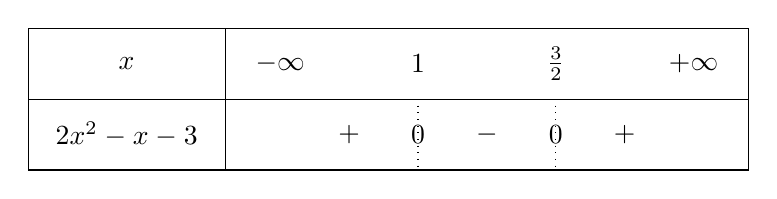
\begin{tikzpicture}[node style/.style={fill opacity=0,text opacity=1}]
        \tkzTabInit[lgt = 2.5, espcl = 1.75, deltacl = 0.7]
        {$x$/.9, $2x^2 - x - 3$/.9}
        {$-\infty$,$1$,$\frac{3}{2}$,$+\infty$}
        \tkzTabLine{,+,z,-,z,+}
    \end{tikzpicture}

\(
\text{Les solutions de l'équation sont :} \quad
\textcolor{red}{\boxed{S=\left]-\infty;\frac{3}{2} \right[ \cup\left] \frac{3}{2};+\infty \right[ }}.
\)
\\
\[ \textbf{c)} \, -3x^2 + 4x - 2 \leq 0 \]

Posons \( -3x^2 + 4x - 2 = 0 \)

\(
\text{Identifions les coefficients :} \quad a = -3, \quad b = 4, \quad c = -2.
\)

\(
\text{Calcul du discriminant } \Delta : \quad
\Delta = b^2 - 4ac = (4)^2 - 4(-3)(-2) = 16 - 24  = -8.
\)

\(
\text{Le discriminant est négatif, donc il y a pas de solutions.}
\)

    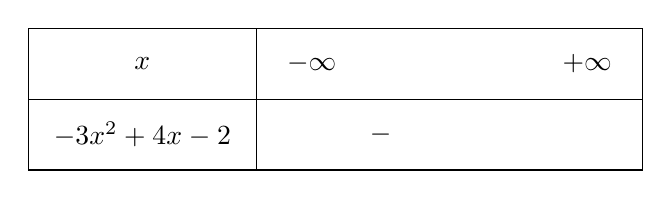
\begin{tikzpicture}[node style/.style={fill opacity=0,text opacity=1}]
        \tkzTabInit[lgt = 2.9, espcl = 1.75, deltacl = 0.7]
        {$x$/.9, $-3x^2 + 4x - 2$/.9}
        {$-\infty$,,$+\infty$}
        \tkzTabLine{,-,}
    \end{tikzpicture}

\(
\text{Les solutions de l'équation sont :} \quad
\textcolor{red}{\boxed{S=\mathbb{R} }}.
\)
\\
\[
\textbf{d)} \, 8x^2 + 34x + 21 < 0
\]

Posons \( 8x^2 + 34x + 21 = 0 \)

\(
\text{Identifions les coefficients :} \quad a = 8, \quad b = 34, \quad c = 21.
\)

\(
\text{Calcul du discriminant } \Delta : \quad
\Delta = b^2 - 4ac = (34)^2 - 4(8)(21) = 1156 - 672  = 484.
\)

\(
\text{Le discriminant est positif, il y a donc deux solutions distinctes.}
\)

\(
\text{Calcul des solutions :} \quad
x = \frac{-b \pm \sqrt{\Delta}}{2a} = \frac{-(34) \pm \sqrt{484}}{2(8)} = \frac{-34 \pm 22}{16}.
\)

\(
\text{Les deux solutions sont :} \quad
x_1 = \frac{-34 + 22}{16} = \frac{6}{16} = \frac{3}{8} \quad \text{et} \quad x_2 = \frac{-34 - 22}{16} = \frac{-56}{16} = \frac{-7}{2}.
\)

    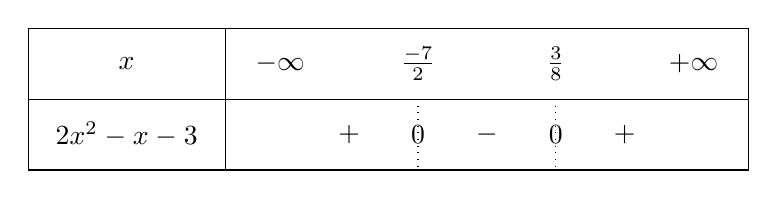
\begin{tikzpicture}[node style/.style={fill opacity=0,text opacity=1}]
        \tkzTabInit[lgt = 2.5, espcl = 1.75, deltacl = 0.7]
        {$x$/.9, $2x^2 - x - 3$/.9}
        {$-\infty$,$\frac{-7}{2}$,$\frac{3}{8}$,$+\infty$}
        \tkzTabLine{,+,z,-,z,+}
    \end{tikzpicture}

\(
\text{Les solutions de l'équation sont :} \quad
\textcolor{red}{\boxed{S=\left]\frac{-7}{2};\frac{3}{8} \right[ }}.
\)
\\

\[ \textbf{e)} \, -9x^2 + 12x - 4 = 0 \]

\(
\text{Identifions les coefficients :} \quad a = -9, \quad b = 12, \quad c = -4.
\)

\(
\text{Calcul du discriminant } \Delta : \quad
\Delta = b^2 - 4ac = (12)^2 - 4(-9)(-4) = 144 - 144 = 0.
\)

\(
\text{Le discriminant est nul, il y a donc une seule solution double.}
\)

\(
\text{Calcul de la solution :} \quad
x = \frac{-b}{2a} = \frac{-12}{2(-9)} = \frac{-12}{-18} = \frac{2}{3}.
\)

\(
\text{La solution de l'équation est :} \quad
\textcolor{red}{\boxed{S=\left\lbrace  \frac{2}{3} \right\rbrace }}.
\)\\

\[ \textbf{f)} \, 4 - 9x^2 = 0 \]

\( \text{Résolvons l'équation :} \quad 4 - 9x^2 = 0 \)

\(
\text{Isolons } x^2 : \quad 9x^2 = 4 \quad \implies \quad x^2 = \frac{4}{9}.
\)

\(
\text{Prenons la racine carrée des deux côtés :} \quad x = \pm \sqrt{\frac{4}{9}} = \pm \frac{2}{3}.
\)

\(
\text{Les solutions de l'équation sont :} \quad
\textcolor{red}{\boxed{S=\left\lbrace  \frac{2}{3},-\frac{2}{3} \right\rbrace }}.
\)


\section*{\underline{Exercice 4 :} 4 points ( Union et Intersection d'Intervalles )}  

\begin{enumerate}
    \item On considère $I = [2, 5]$ et $J = [4, 7]$ :
    \begin{itemize}
        \item $I \cup J = [2, 7]$
        \item $I \cap J = [4, 5]$
    \end{itemize}

    \item On considère $K = [2, 5]$ et $L = [6, 7]$ :
    \begin{itemize}
        \item $K \cap L = \varnothing$
        
 \(
 \quad
\textcolor{red}{\boxed{K \cap L = \varnothing  }}.
\)
    \end{itemize}
\end{enumerate}
\end{document}
